% id: 108-26
% book: 쎈B 공통수학1 · 09 순열과 조합
% section: 유형 07 색칠하는 경우의 수
% figure: tikz:fig-108-26
% answer: 
% answer_source: 
% variant_level: 0 (원본 전사)
% 이 파일은 build.mjs 가 items.json 에서 만든다. 고칠 때는 items.json 을 고친다.
\smash{\raisebox{1.5mm}{\dmkichul{쎈B 공통수학1 108쪽 26번}}}
\noindent\begin{minipage}[t]{0.58\linewidth}\vspace{0pt}\raggedright 오른쪽 그림의 6개의 영역을 서로 다른 5가지 색으로 칠하려고 한다. A, B, C, D, E, F의 영역에 같은 색을 중복하여 사용해도 좋으나 인접한 영역은 서로 다른 색으로 칠할 때, 칠하는 경우의 수는? \dmcondfill{각 영역에는 한 가지 색만 칠한다.}{}\end{minipage}\hfill\begin{minipage}[t]{0.4\linewidth}\vspace{0pt}\centering \resizebox{\ifdim\width>\linewidth\linewidth\else\width\fi}{!}{% 108-26(108쪽) — 큰 직사각형 안에 작은 직사각형을 넣고 네 꼭짓점을 이어 만든 6개의 영역 A, B, C, D, E, F. 스캔 그림이라 TikZ 로 다시 그림.
% 라벨은 원문 그대로 A~F 만. 가운데 직사각형은 세로선으로 A(왼쪽)·B(오른쪽)로 나뉜다.
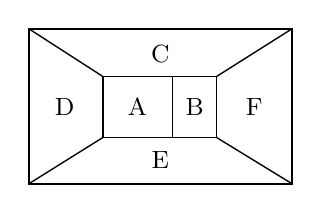
\begin{tikzpicture}[scale=0.62, line width=0.5pt]
  \def\ox{5.4}\def\oy{3.18}
  \def\ix{1.52}\def\jx{3.85}\def\iy{0.95}\def\jy{2.20}
  \draw[line width=0.7pt] (0,0) rectangle (\ox,\oy);
  \draw (0,\oy) -- (\ix,\jy);
  \draw (\ox,\oy) -- (\jx,\jy);
  \draw (0,0) -- (\ix,\iy);
  \draw (\ox,0) -- (\jx,\iy);
  \draw (\ix,\iy) rectangle (\jx,\jy);
  \draw (2.95,\iy) -- (2.95,\jy);
  \node[font=\small] at (2.70,2.66) {$\mathrm{C}$};
  \node[font=\small] at (0.74,1.58) {$\mathrm{D}$};
  \node[font=\small] at (2.70,0.49) {$\mathrm{E}$};
  \node[font=\small] at (4.62,1.58) {$\mathrm{F}$};
  \node[font=\small] at (2.23,1.58) {$\mathrm{A}$};
  \node[font=\small] at (3.40,1.58) {$\mathrm{B}$};
\end{tikzpicture}
}\end{minipage}\par
\dmchoicesauto{}{$900$}{$960$}{$1020$}{$1080$}{$1140$}
